\subsection{Opis zadania}
Celem tego zadania było wykorzystanie wstępnie wytrenowanej sieci do uczenia wyłącznie części klasyfikującej (ostatnich warstw o połączeniach kompletnych). Następnie wyniki klasyfikacji zostały przeanalizowane. Kolejnym krokiem było zastąpienie części klasyfikującej sieci klasyfikatorem SVM z różnymi jądrami: liniowym, kwadratowym (poly) oraz RBF. Wyniki klasyfikacji dla każdego jądra zostały porównane, a szczególna uwaga została poświęcona efektowi dopuszczenia błędnych klasyfikacji.

\subsection{Wybór architektury modelu}
Do realizacji zadania wykorzystano sieć EfficientNetB0, wstępnie wytrenowaną na zbiorze ImageNet. Warstwy bazowe modelu zostały zamrożone, aby nie były aktualizowane podczas uczenia. Ostatnie warstwy klasyfikujące zostały zastąpione następującą strukturą:
\begin{itemize}
    \item Warstwa GlobalAveragePooling2D,
    \item Warstwa Dropout (z prawdopodobieństwem $0.2$),
    \item Warstwa Dense z liczbą neuronów odpowiadającą liczbie klas i funkcją aktywacji softmax.
\end{itemize}

\noindent Struktura modelu została przedstawiona w Tabeli~\ref{tab:model_summary}.
\begin{table}[h!]
\centering
\begin{tabular}{|l|l|l|}
\hline
\textbf{Warstwa}                  & \textbf{Rozmiar wyjścia}       & \textbf{Liczba parametrów} \\ \hline
Wejście                          & (None, 224, 224, 3)           & 0                          \\ \hline
EfficientNetB0                   & (None, 7, 7, 1280)            & 4,049,571                  \\ \hline
GlobalAveragePooling2D           & (None, 1280)                  & 0                          \\ \hline
Dropout                          & (None, 1280)                  & 0                          \\ \hline
Dense                            & (None, 4)                     & 5,124                      \\ \hline
\end{tabular}
\caption{Podsumowanie modelu klasyfikatora.}
\label{tab:model_summary}
\end{table}

\subsection{Wyniki uczenia klasyfikatora}
Wyniki procesu uczenia, przedstawione na wykresach (Rys.~\ref{fig:loss_accuracy}), ilustrują zmniejszanie się wartości funkcji straty (loss) oraz wzrost dokładności (accuracy) w zbiorach treningowym i walidacyjnym.

\begin{figure}[h!]
    \centering
    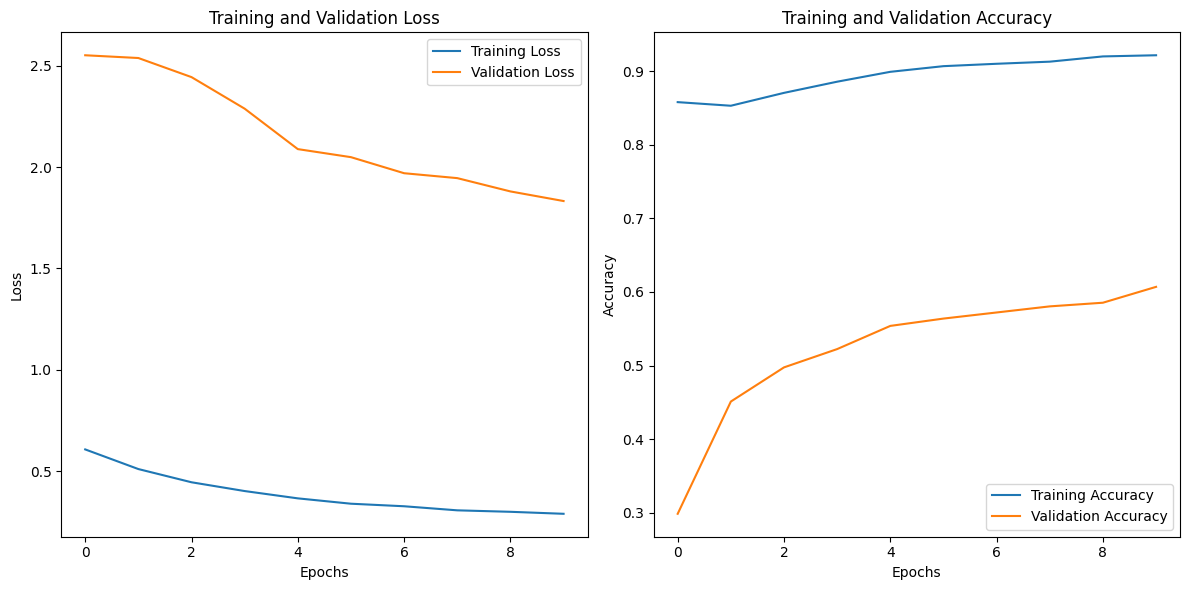
\includegraphics[width=0.9\textwidth]{img/loss.png}
    \caption{Wykresy funkcji straty i dokładności dla zbiorów treningowego i walidacyjnego.}
    \label{fig:loss_accuracy}
\end{figure}

\begin{table}[h!]
\centering
\begin{tabular}{|c|c|c|c|c|}
\hline
\textbf{} & \textbf{Klasa 0} & \textbf{Klasa 1} & \textbf{Klasa 2} & \textbf{Klasa 3} \\ \hline
\textbf{Klasa 0} & 41 & 39 & 46 & 2 \\ \hline
\textbf{Klasa 1} & 26 & 206 & 2 & 0 \\ \hline
\textbf{Klasa 2} & 4 & 7 & 97 & 3 \\ \hline
\textbf{Klasa 3} & 29 & 51 & 32 & 11 \\ \hline
\end{tabular}
\caption{Macierz pomyłek dla zbioru testowego.}
\label{tab:confusion_matrix_last_layer}
\end{table}

\subsection{Zastąpienie klasyfikatora sieci SVM}
W celu poprawy klasyfikacji, cechy wyodrębnione z ostatniej warstwy modelu EfficientNetB0 zostały wykorzystane do uczenia klasyfikatora SVM z różnymi jądrami. Wyniki klasyfikacji zostały ocenione za pomocą miar takich jak precision, recall i F1-score.

\subsubsection{Wyniki dla różnych jąder}
\begin{itemize}
    \item \textbf{Jądro liniowe:} Dokładność wyniosła $88\%$, a F1-score dla poszczególnych klas mieściło się w zakresie $0.80$--$0.95$. 
    \item \textbf{Jądro kwadratowe (poly):} Najwyższa dokładność na poziomie $93\%$, przy wysokich wartościach precision i recall.
    \item \textbf{Jądro RBF:} Dokładność również wyniosła $93\%$, jednak efektywność była różna w zależności od klasy.
\end{itemize}

\subsubsection{Macierze pomyłek}
Macierze pomyłek dla każdego jądra pozwoliły na identyfikację klas trudniejszych do rozróżnienia, co przedstawiono na rysunku~\ref{fig:confusion_matrix}.
\begin{figure}[h!]
    \centering
    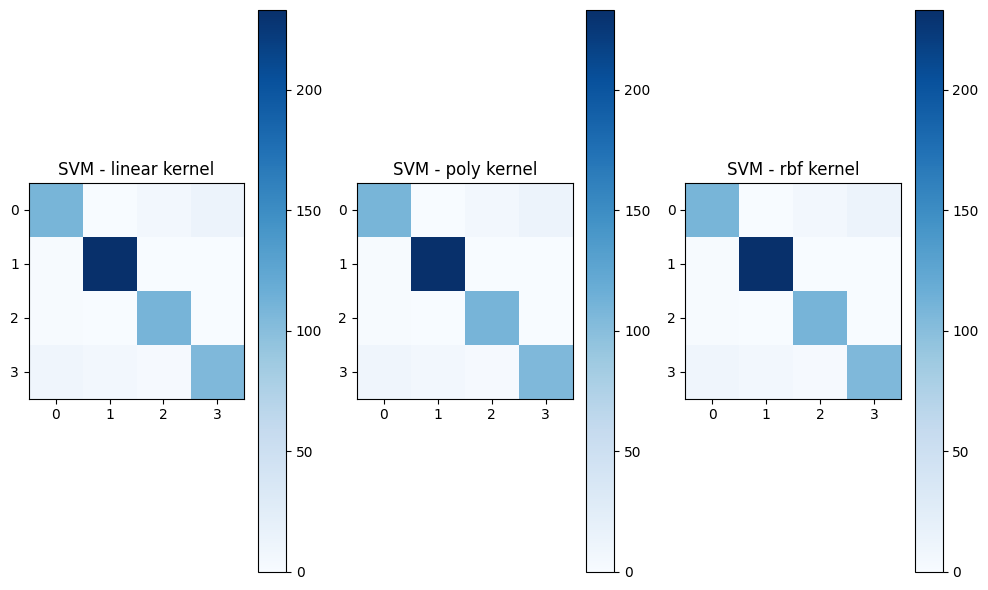
\includegraphics[width=0.9\textwidth]{img/svm.png}
    \caption{Macierze pomyłek dla różnych jąder SVM.}
    \label{fig:confusion_matrix}
\end{figure}

\subsection{Podsumowanie}
Porównanie wyników klasyfikacji dla różnych jąder SVM wykazało, że jądra kwadratowe i RBF osiągają wyższą dokładność niż jądro liniowe, co sugeruje lepsze odwzorowanie granic decyzyjnych w bardziej złożonych przestrzeniach. Wyniki te wskazują na możliwość dalszej poprawy wydajności modelu poprzez dostrojenie hiperparametrów klasyfikatora.
